\section{Implementation}

\begin{figure}[H]
  \label{fig:devops}
  \centering
  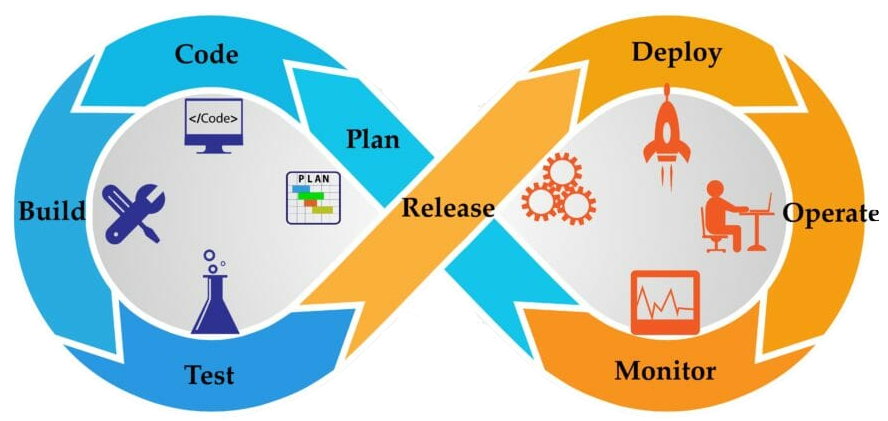
\includegraphics[scale=0.35]{images/devops.png}
  \caption{DevOps approach.}
\end{figure}

The implementation follow the \textbf{DevOps approach}.
According to this model, the developer and operation teams work together, across the entire lifecycle, from the development/deployment to test operations.
This approach entails a lot of benefits:
\begin{itemize}
\item \textbf{speed}: quickly it adapts to market needs and perform faster the implementation of the new features; 
\item \textbf{rapid delivery}: it consists in light and frequent updates in order to fix any bugs and make the application more secure in case of vulnerability.
The frequent update makes easy finding and fixing any bugs;
\item \textbf{scalability}: the DevOps approach helps us to manage our development, testing, and production environments in a repeatable and more efficient manner;
\item the use of \textbf{microservices}, which are indipendent from each other and from the system, helps to implement new features and allow to modify only the component involved.
\end{itemize}



\section{Integration}
We'll use the following ones, which are the main methods for a DevOps approach. These improve developers interactions and reduce time for next releases.
\bigskip

\textbf{Continuous integration}
Continuous integration is a software development practice where developers regularly update any code modification into the main branch of the central repository as often as possible. In this way builds are created and test runned due to a better collaboration. The target of CI is to find potential bugs quicker, improve software quality, and reduce the time it takes to validate and release new software updates.
\par
\textbf{Continuous Delivery} 
CD is an extension of continous integration where, instead, code changes are automatically built, tested, and prepared for releases. In this way, developers will always have a deployment-ready build artifact to run. It also includes unit test in order to automate testing which improve productivity. Moreover, bugs are solved with more readiness.
\par

It will be used \textbf{Git}, an open source distributed version control system, as source control and \textbf{Jenkins} as continuous integration.
Jenkins is a popular open source tool to perform continuous integration and build automation.
It also monitors the execution of the steps and allows to stop the process, if one of the steps fails. Jenkins can also send out notification in case of a successfull or failure build.

 
\section{Testing}

\textbf{Continuous Testing} needs to be a key element in DevOps approach for a right implementation. \\
This is a procedure in which testing is performed earlier in the software lifecycle, by increasing quality, shortening long test cycles and reducing defects in software.
This is necessary with DevOps because software moves continuously from development to testing to deployment.
\par
Another important aspect of testing a product software is the \textbf{Quality Assurance}.
QA testing is the process that ensures the best quality possibile of the software developed. This is made by combining automated tests and manual testing. 
In our case, QA is required to be aligned with respect to a DevOps cycle.
This is due to the fact that DevOps don't have to check software quality as an external entity. QA infact will be a part of the development process made by each team. 
So testers have to work very close to developers to collaborate on testing for the entire software development lifecycle.














\begin{comment}
For istance, we have to make sure that all their test cases are automated and that they achieve near 100\% code coverage.\\
To improve speed and agility, it needs to automate all the testing processes and configure them to run automatically.  


 

The test cases that are required to be executed for a particular build need to be identified.
The QA and Dev need to sit together and identify the areas affected due to a particular build and execute those related test cases plus a sanity test pass.
You also need to configure specialized code analysis and coverage tools to make sure that you achieve near 100% code coverage.
The concept of executing all regression test cases for a test pass is soon becoming obsolete.
The strategy around testing new features needs to be formalized and the interim builds can be supplied to QA who would, in turn, create test scr
ipts and run these automation tests on the interim builds till the code becomes stable enough to be deployed onto the Production environment.
All the environments required for testing need to be standardized and the deployments have to be automated.
Using various automation techniques, QA should be able to fire Automation Testing runs across various cross-platform (and cross-browser in case of web applications) environments.
Exit criteria need to be set for each run so that when the results of the tests are fed back to the chain, a go/no-go decision to Production is taken.
Blocker or Critical bugs found need to be reported, fixed and passed through the same chain of events before the code is deployed in the Production environment.
\end{comment}